\documentclass[resume]{subfiles}


\begin{document}
    \section{Équations non linéaires}
	\subsection{Existence d'une solution}
	Solution $f(r)=0$ entre $a$ et $b$ pour $f$ continue
	$$f(a)\cdot f(b)<0$$
	\subsection{Bissection}
	\begin{enumerate}
	\item $a_0=a$, $b_0=b$, $x_0=\frac{a+b}{2}$
	\item Répéter jusqu'à ce que $\abs{a_k-b_k}\geq tol\cdot \abs{b_k}$
	\begin{enumerate}
	\item Si $f(x_k)f(a_k)<0$ : $a_{k+1}=a_k$, $b_{k+1}=x_k$
	\item Si $f(x_k)f(a_k)>0$ : $a_{k+1}=x_k$, $b_{k+1}=b_k$
	\item $x_{k}=\frac{a_{k}+b_{k}}{2}$
	\end{enumerate}
	\end{enumerate}
	L'erreur converge avec
	$$\abs{e_k}<\frac{b-a}{2^{k+1}}$$
	\begin{enumerate}
	\item Robuste
	\item Intervalles qui contiennent la solution
	\item Majorant connu de l'erreur
	\item Lente
	\end{enumerate}
	\subsection{Regula falsi}
A l'exception du premier terme, on doit décider si on utilise $x_{k-1}$ avec $x_{k-2}$ ou $x_{k-3}$
$$\boxed{x_{k}=\begin{cases}
x_{k-2}-y_{k-2}\frac{x_{k-1}-x_{k-2}}{y_{k-1}-y_{k-2}} & y_{k-1}\cdot y_{k-2} < 0\\
x_{k-3}-y_{k-3}\frac{x_{k-1}-x_{k-3}}{y_{k-1}-y_{k-3}} & y_{k-1}\cdot y_{k-3} < 0
\end{cases}}$$
\subsection{Sécante}
$$\boxed{x_{k+1}=x_{k}-f(x_k)\frac{x_k-x_{k-1}}{f(x_k)-f(x_{k-1})}}$$
Ordre de convergence de
$$p=\frac{1+\sqrt{5}}{2}=\phi$$
\begin{enumerate}
\item Pas de connaissance de la dérivée
\item Une seule évaluation de $f$
\item Plus efficace que Newton (plus facile à calculer)
\item Convergence non garantie
\end{enumerate}
\subsection{Newton}
$$\boxed{x_{k+1}=x_{k}-\frac{f(x_{k})}{f'(x_{k})}}$$
$$\abs{e_{k+1}}\approx \abs{\frac{f''(r)}{f'(r)}}\cdot \abs{e_k}^2$$
\begin{enumerate}
\item Très rapide
\item Peut ne pas converger
\item Utilisation de la dérivée
\end{enumerate}
\subsection{Point fixe}
$$\boxed{x=F(x)}$$
Résultat global mais difficile de trouver un domaine $D$... Il existe une version locale
$$\rho(\mathbf{J}(\mathbf{r}))<1\longrightarrow\text{ converge dans un disque } D\text{ vers }\mathbf{r}$$
Avec $\rho$ le rayon spectral (maximum des modules des valeurs propres de la matrice).
\subsubsection{Théorème de Banach}
$$\max_{x\in I}\abs{F'(x)}<1\longrightarrow\text{ contraction sur }I$$
$$\abs{F(x_1)-F(x_2)}\leq L\abs{x_1-x_2}$$
$$0<L<1\quad \forall x_1,x_2\in I$$
Alors il existe une seule solution $r$ dans $I$
\begin{enumerate}
\item Fonction Lipschitzienne : qui satisfait la condition de Lipschitz avec n'importe quel $L$
\item Fonction contractante : qui satisfait la condition de Lipschitz et $0<L<1$
\end{enumerate}
$$L_\text{optimal}=\max_{x\in I}\abs{F'(x)}$$
\subsubsection{Estimation}
\begin{enumerate}
\item A priori : 
$$\abs{\abs{\mathbf{r}-\mathbf{x}_k}}\leq \frac{L^{k}}{1-L}\abs{\mathbf{x}_1-\mathbf{x}_0}$$
\item A posteriori :
$$\abs{\abs{\mathbf{r}-\mathbf{x}_k}}\leq \frac{L}{1-L}\abs{\mathbf{x}_k-\mathbf{x}_{k-1}}$$
\end{enumerate}

\section{Systèmes d'équations non-linéaires}
\subsection{Point fixe}
$$\boxed{\mathbf{F}(\mathbf{x})=\begin{pmatrix}
F(x,y)\\
G(x,y)
\end{pmatrix}\qquad \mathbf{x}=\begin{pmatrix}
x\\y
\end{pmatrix}}$$
$\mathbf{F}$ est une contraction si
$$\abs{\abs{\mathbf{F}(\mathbf{x})-\mathbf{F}(x')}}\leq L\abs{\abs{\mathbf{x}-\mathbf{x}'}}\qquad \abs{\abs{\mathbf{x}}}=\sqrt{x^2+y^2}$$
Et donc $\mathbf{F}$ possède un seul point fixe (et y converge de toute façon).
$$\boxed{\max_{(x,y)\in D}\abs{\abs{\mathbf{J}(x,y)}}<1\longrightarrow \text{ contraction sur }D}$$
\begin{scriptsize}
$$\abs{\abs{\mathbf{J}(x,y)}}=\sqrt{F_x(x,y)^2+F_y(x,y)^2+G_x(x,y)^2+G_y(x,y)^2}$$
\end{scriptsize}
Matrice de Jacobi :
$$\mathbf{J}(x,y)=\begin{pmatrix}
F_x(x,y) & F_y(x,y)\\
G_x(x,y) & G_y(x,y)
\end{pmatrix}$$
\subsection{Méthode de Newton}
\begin{small}
$$\boxed{x_{k+1}=x_k+\frac{g(x_k,y_k)f_y(x_k,y_k)-f(x_k,y_k)g_y(x_k,y_k)}{f_x(x_k,y_k)g_y(x_k,y_k)-f_y(x_k,y_k)g_x(x_k,y_k)}}$$
$$\boxed{y_{k+1}=y_k+\frac{f(x_k,y_k)g_x(x_k,y_k)-g(x_k,y_k)f_x(x_k,y_k)}{f_x(x_k,y_k)g_y(x_k,y_k)-f_y(x_k,y_k)g_x(x_k,y_k)}}$$
\end{small}
\begin{figure}[H]
\centering
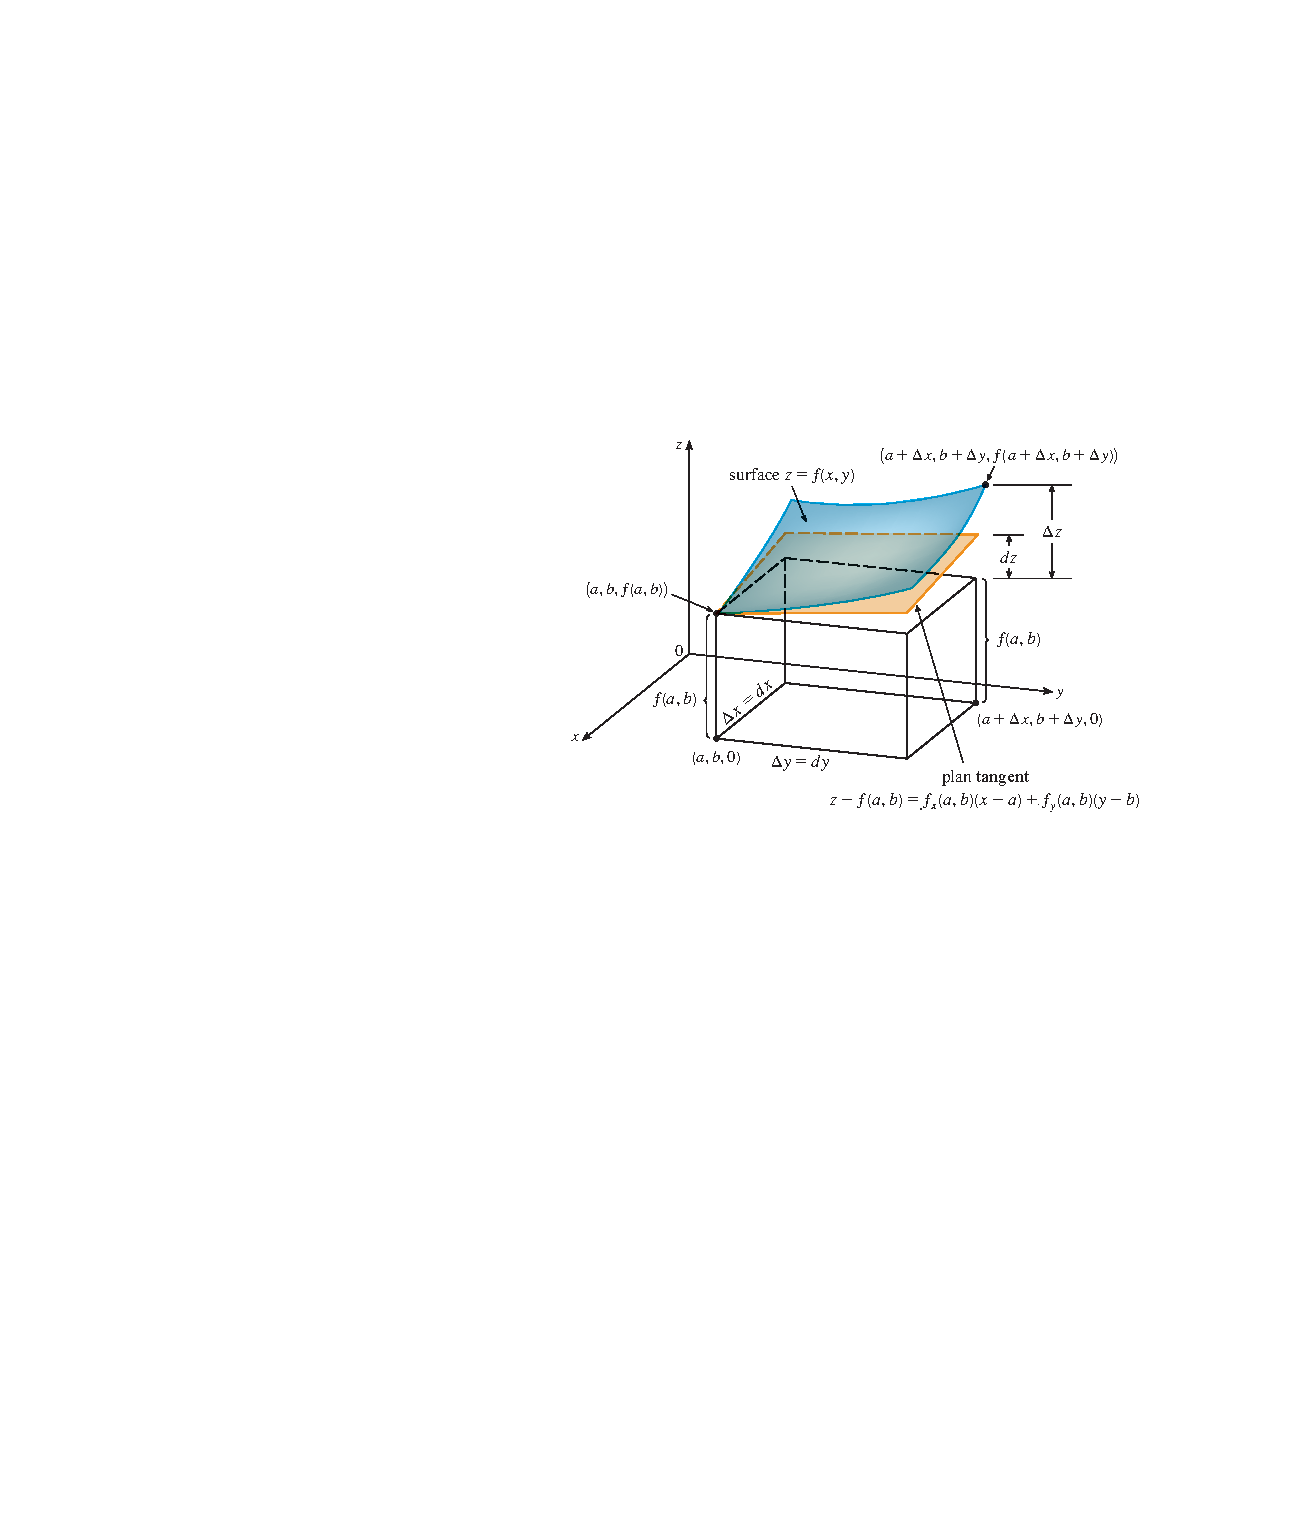
\includegraphics[width=0.8\columnwidth]{img_18.pdf}
\end{figure}
La matrice de Jacobi donne une information sur la convergence (lente si déterminant égal à 0)
\subsubsection{Ordre}
Convergence linéaire
$$\abs{\abs{\mathbf{e}_{k+1}}}\lessapprox \abs{\abs{\mathbf{J}(r,s)}}\cdot \abs{\abs{\mathbf{e}_k}}$$
Si $\mathbf{J}(r,s)$ est nulle on a un ordre de convergence quadratique.
	


    
\end{document}